\section{Atomic Data Types}
\begin{frame}{Objects}
    \begin{itemize}
        \item Everything in Python is an object
        \item Objects have attributes and methods
        \item Objects can be created from classes
        \item Classes define the attributes and methods of objects
    \end{itemize}
\end{frame}
\begin{frame}
    \begin{figure}
        \centering
        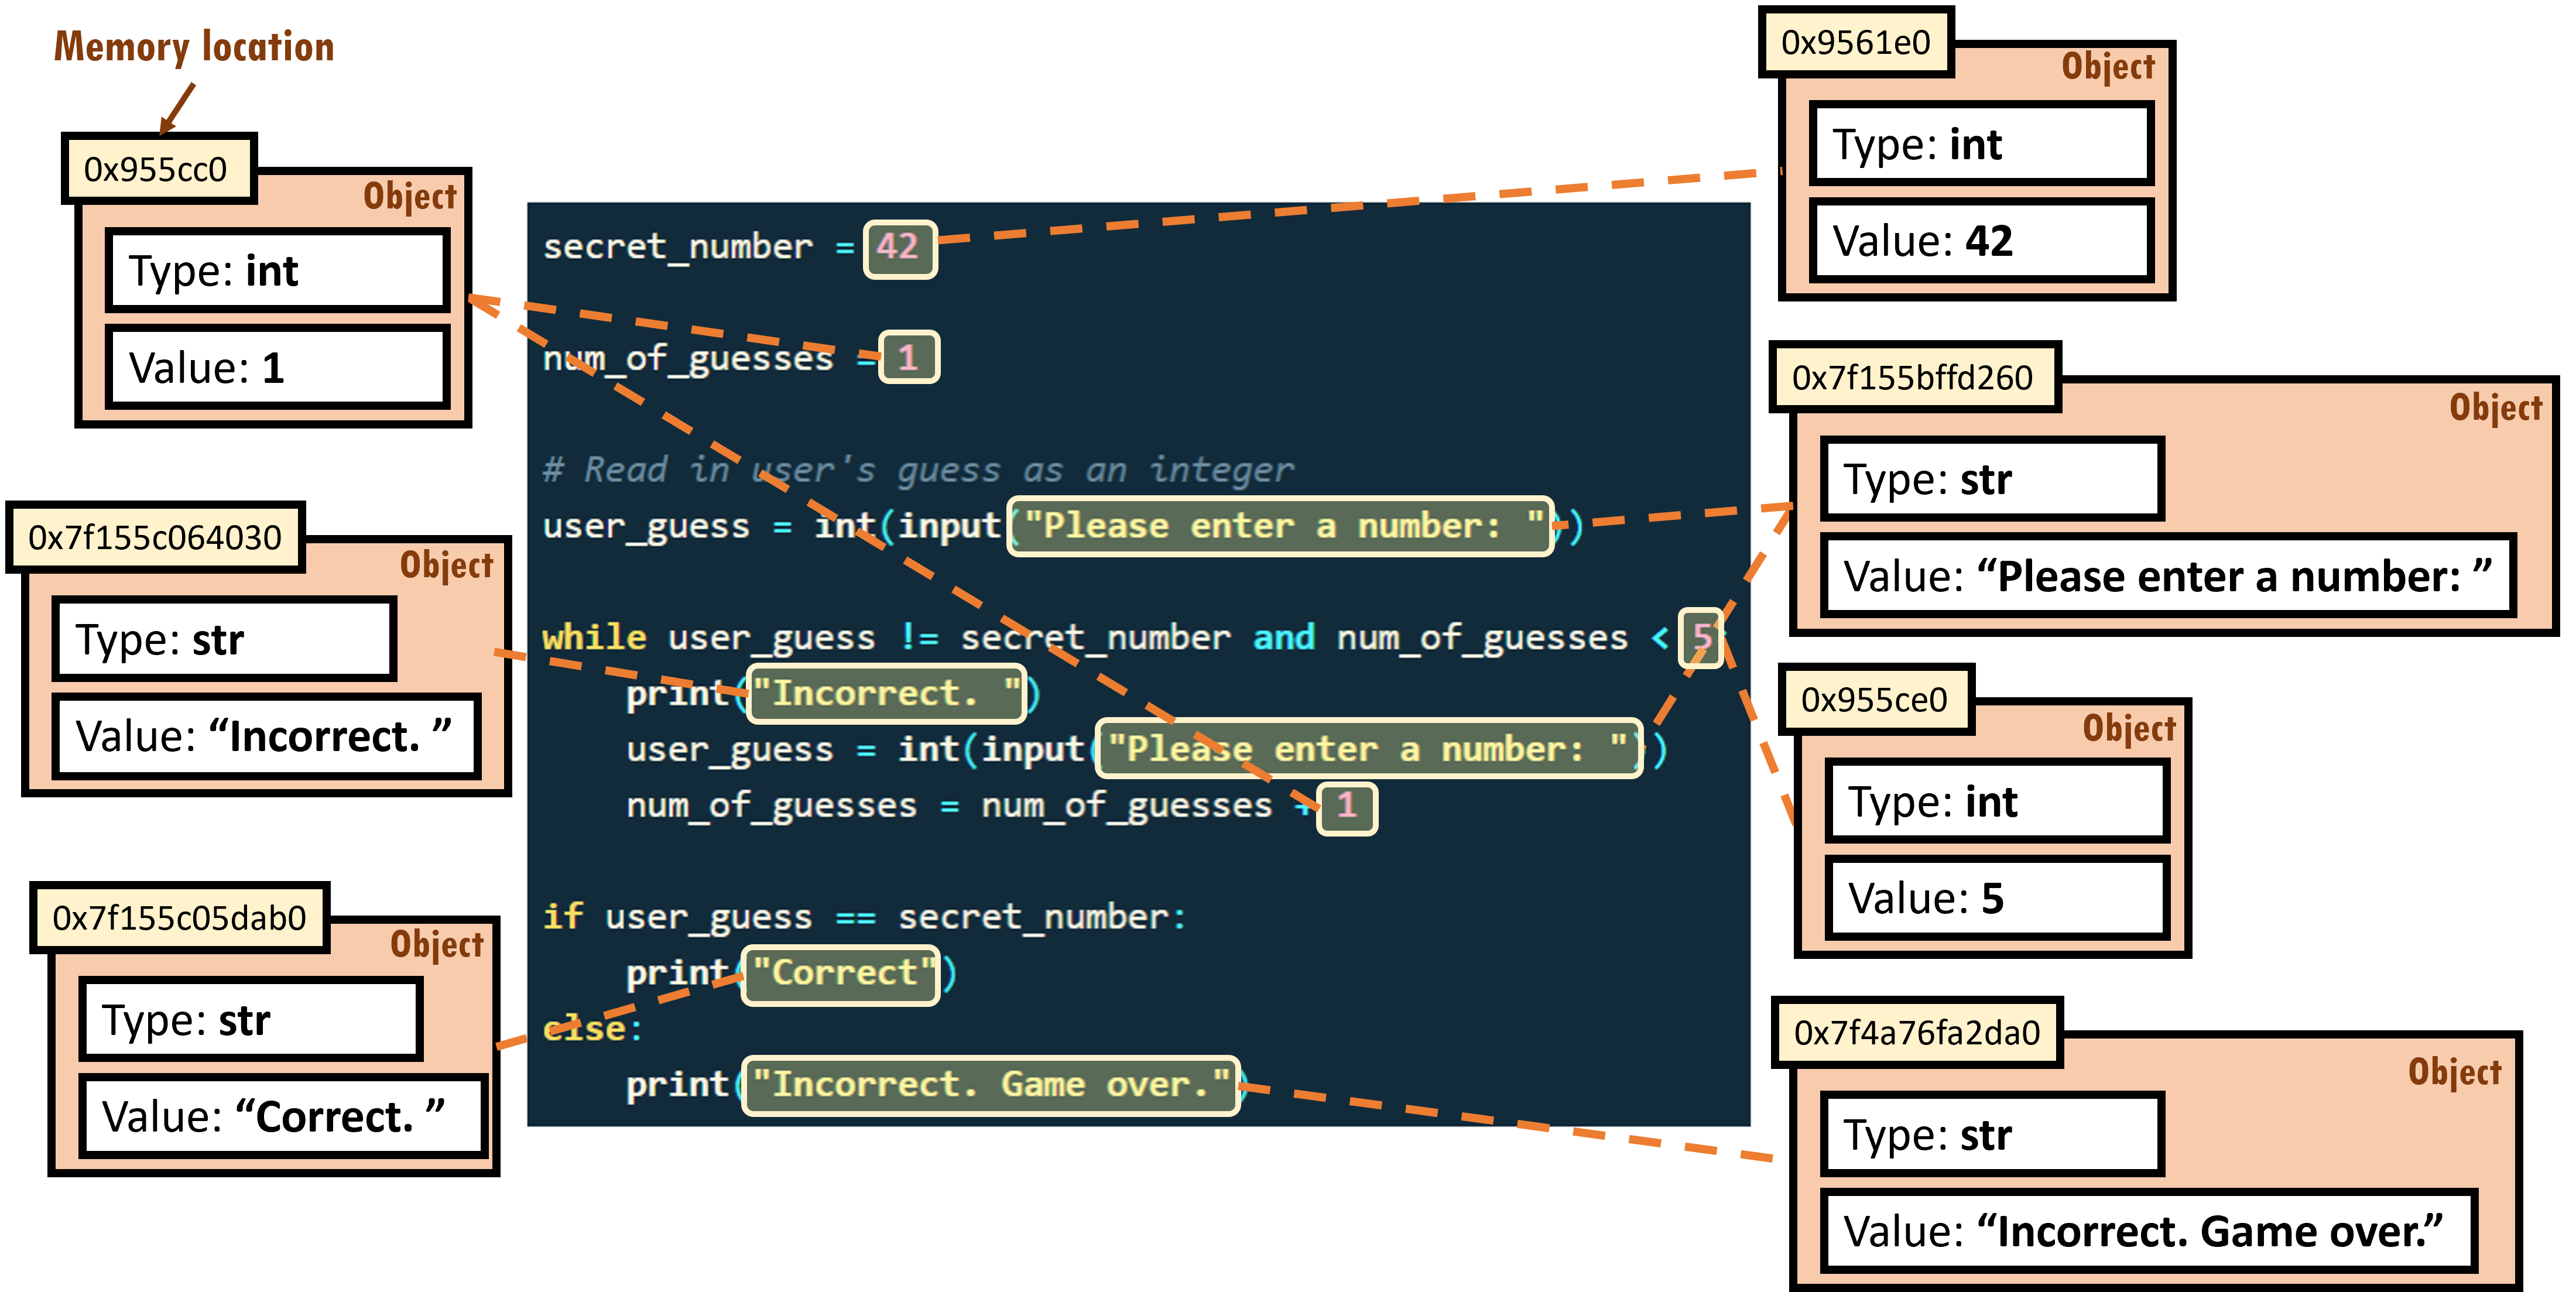
\includegraphics[width=1.0\textwidth]{pics/objects.png}
        \caption{Objects in Python}
    \end{figure}
\end{frame}
\begin{frame}{Built in atomic datatypes}
    \begin{itemize}
        \item Python provides built-in data types
        \item These types are used to represent data in programs
        \item Common data types include:
        \begin{itemize}
            \item Integers
            \item Floats
            \item Strings
            \item Booleans
        \end{itemize}
    \end{itemize}
\end{frame}
\begin{frame}{Operators and Expressions}
    \begin{columns}
        \column{0.5\textwidth}
        \begin{itemize}
            \item Objects can be combined using operators
            \item Arithmrtic operators in python 
            \begin{itemize}
            \item \texttt{+} (addition)
            \item \texttt{-} (subtraction)
            \item \texttt{*} (multiplication)
            \item \texttt{/} (division)
            \item \texttt{//} (floor division, or integer part of division)
            \item \texttt{\%} (modulo, or remainder after division)
            \item \texttt{**} (exponential -- raised to the power)
            \end{itemize}
                    \end{itemize}
        \column{0.5\textwidth}
        \begin{figure}
            \centering
            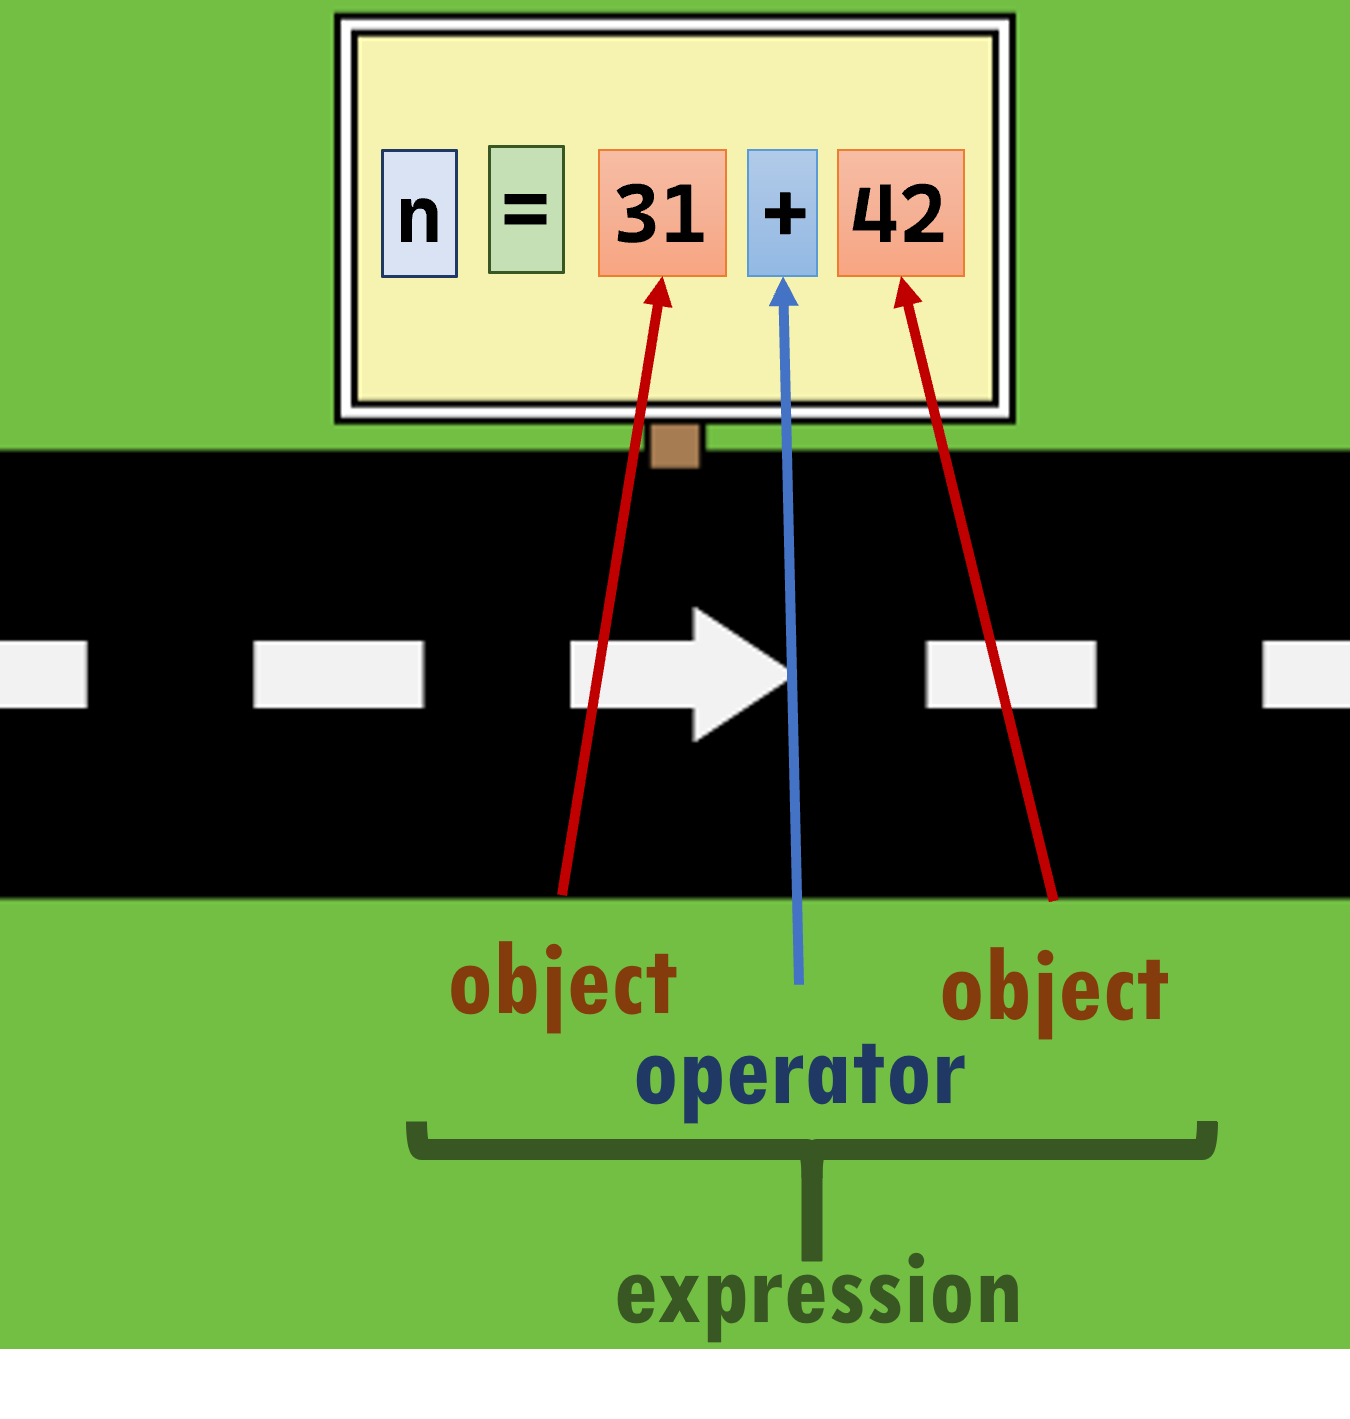
\includegraphics[width=0.8\textwidth]{pics/operator.png}
            \caption{Operators in Python}
        \end{figure}
    \end{columns}
\end{frame}
\begin{frame}{Python Operator Precedence}
    \begin{itemize}
        \item Python evaluates expressions based on operator precedence.
        \item Common operators in order of precedence (from highest to lowest):
        \begin{itemize}
            \item \texttt{()} -- Parentheses
            \item \texttt{**} -- Exponentiation
            \item \texttt{+x}, \texttt{-x}, \texttt{\textasciitilde{}x} -- Unary plus, Unary minus, Bitwise NOT
            \item \texttt{*}, \texttt{/}, \texttt{//}, \texttt{\%} -- Multiplication, Division, Floor division, Modulus
            \item \texttt{+}, \texttt{-} -- Addition, Subtraction
            \item \texttt{<<}, \texttt{>>} -- Bitwise shift operators
            \item \texttt{\&} -- Bitwise AND
            \item \texttt{\textasciicircum} -- Bitwise XOR
            \item \texttt{|} -- Bitwise OR
            \item \texttt{==}, \texttt{!=}, \texttt{>}, \texttt{<}, \texttt{>=}, \texttt{<=}, \texttt{is}, \texttt{is not}, \texttt{in}, \texttt{not in} -- Comparisons, Identity, Membership
            \item \texttt{not} -- Logical NOT
            \item \texttt{and} -- Logical AND
            \item \texttt{or} -- Logical OR
        \end{itemize}
        \item Example: \texttt{1 + 2 * 3 == 7} evaluates as \texttt{1 + (2 * 3) == 7}, which is \texttt{1 + 6 == 7}, resulting in \texttt{True}.
    \end{itemize}
\end{frame}
\begin{frame}[fragile]{Overloaded Operators}
    \begin{itemize}
        \item Some operators are not limited to arithmetic operations with numbers.
        \item For example, \texttt{+} and \texttt{*} can be used for a different kind of operation when used with strings.
    \end{itemize}
    \begin{lstlisting}[style=colorful, language=Python]
>>> 'hello' + 'world'
'helloworld'
>>> 'hello' * 3
'hellohellohello'
    \end{lstlisting}
\end{frame}

\begin{frame}{Variables}
    In Python, a variable is simply a name or a label that points to an object instance in memory
    \begin{figure}
        \centering
        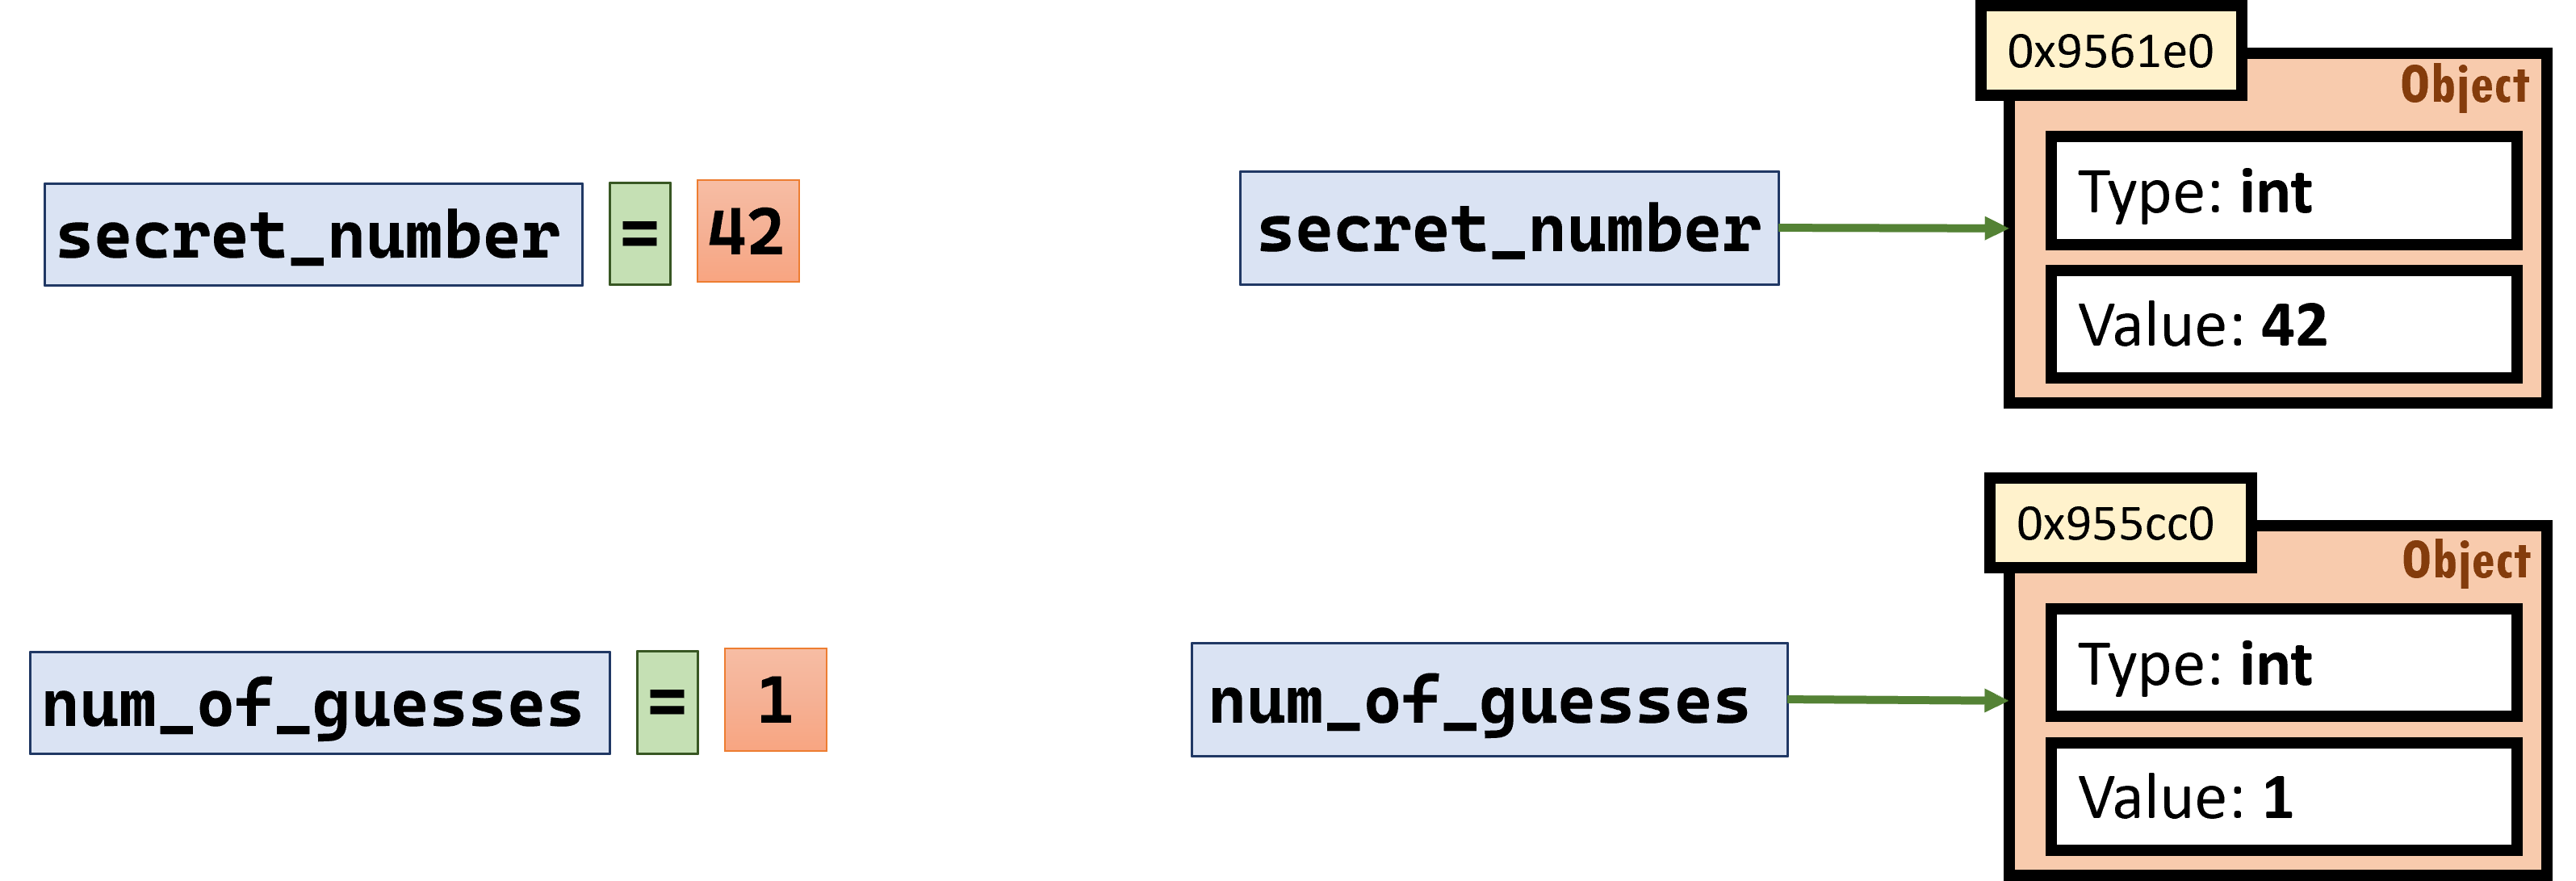
\includegraphics[width=0.8\textwidth]{pics/variable.png}
        \caption{Variables in Python}
    \end{figure}
\end{frame}

\begin{frame}{Variable Assignments}
    \begin{columns}
        \column{0.5\textwidth}
        \begin{figure}
            \centering
            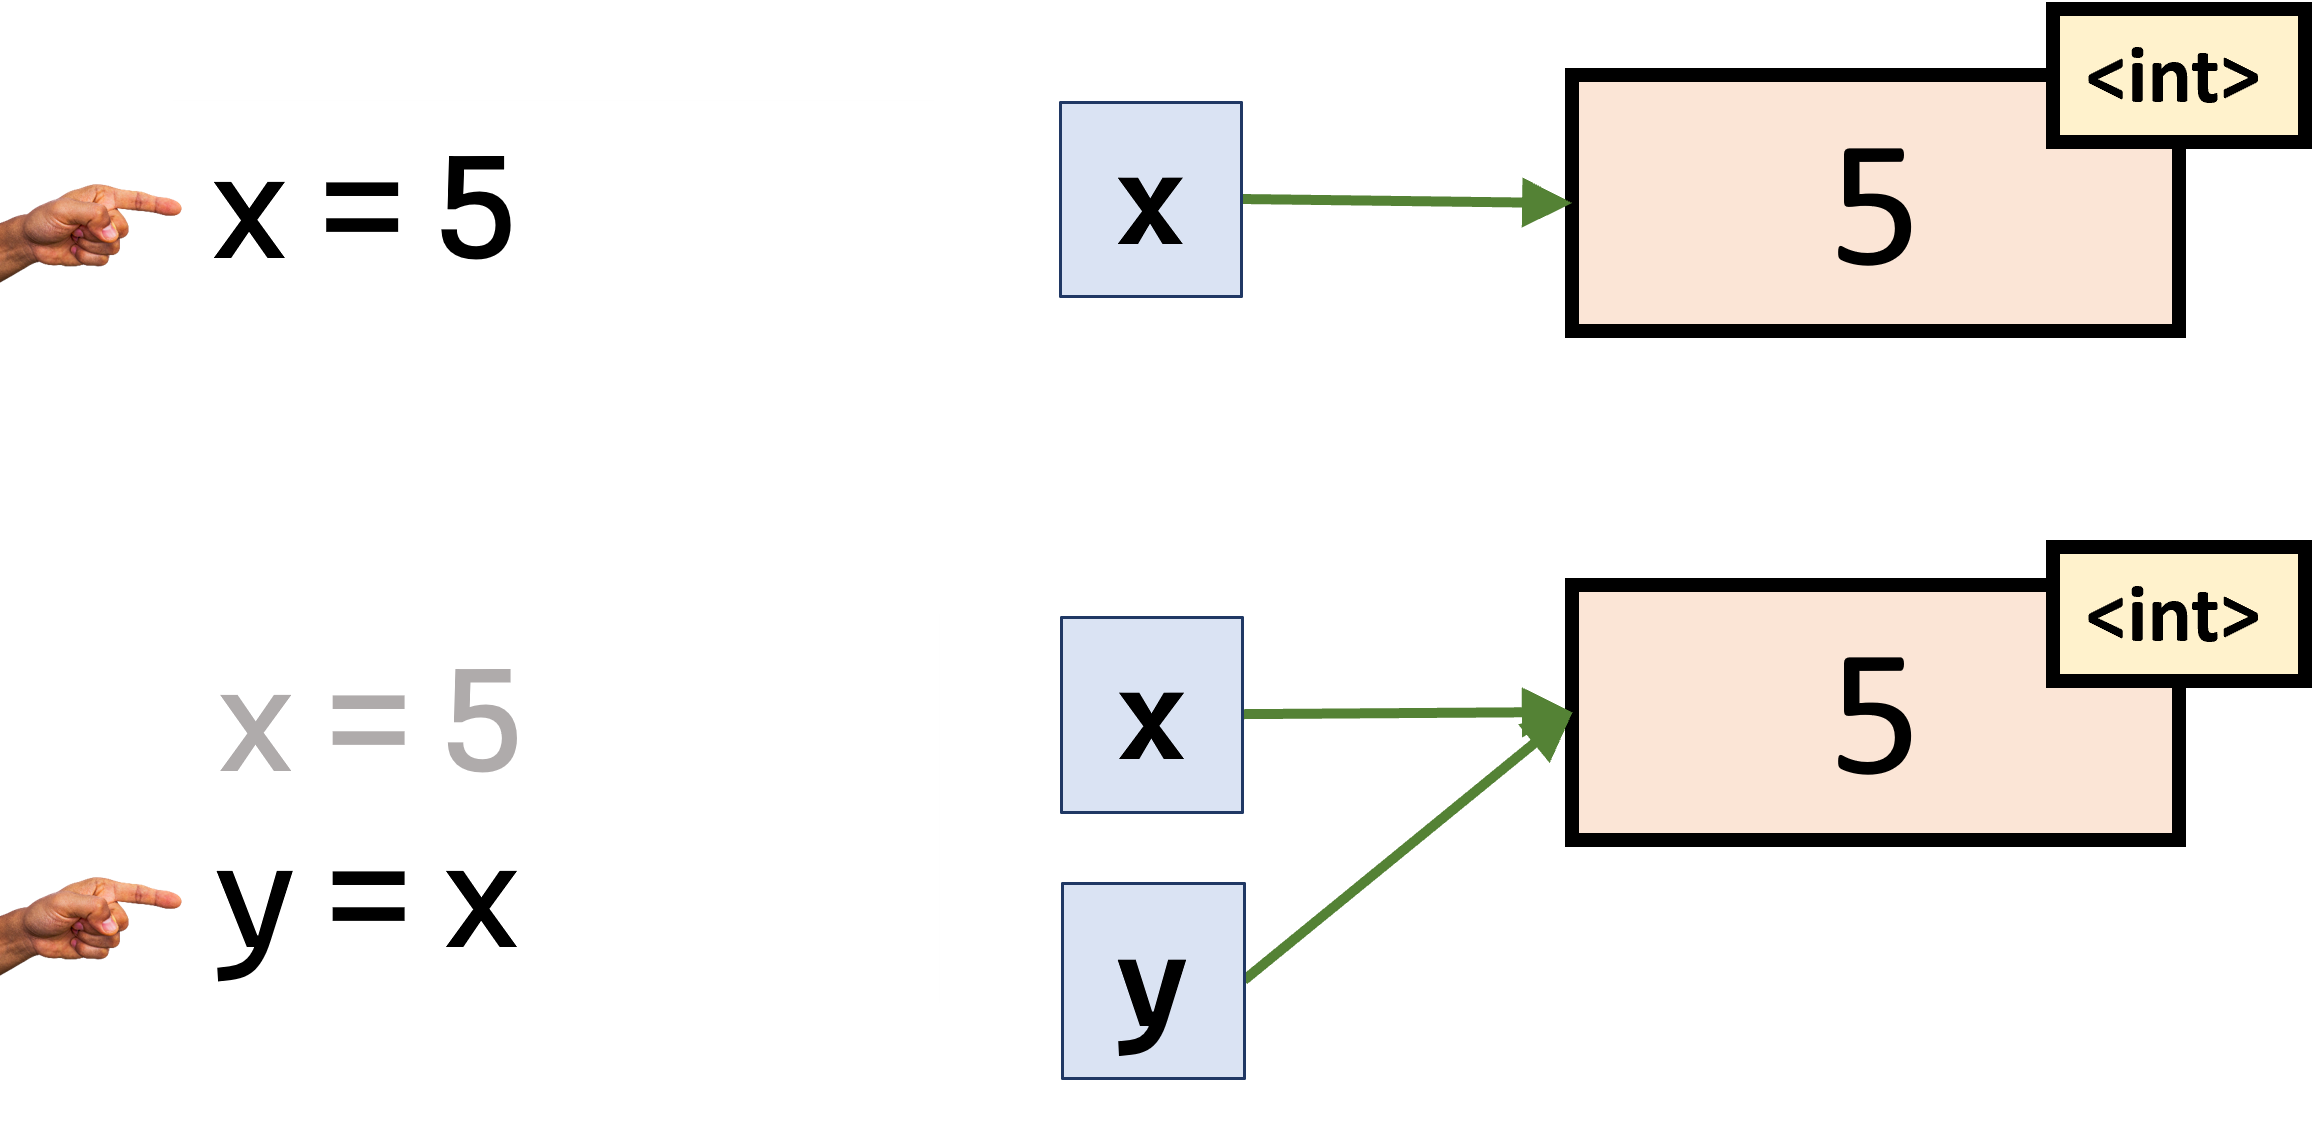
\includegraphics[width=0.8\textwidth]{pics/assignment.png}
            \caption{Variable Assignment}
        \end{figure}
        \column{0.5\textwidth}
        \begin{figure}
            \centering
            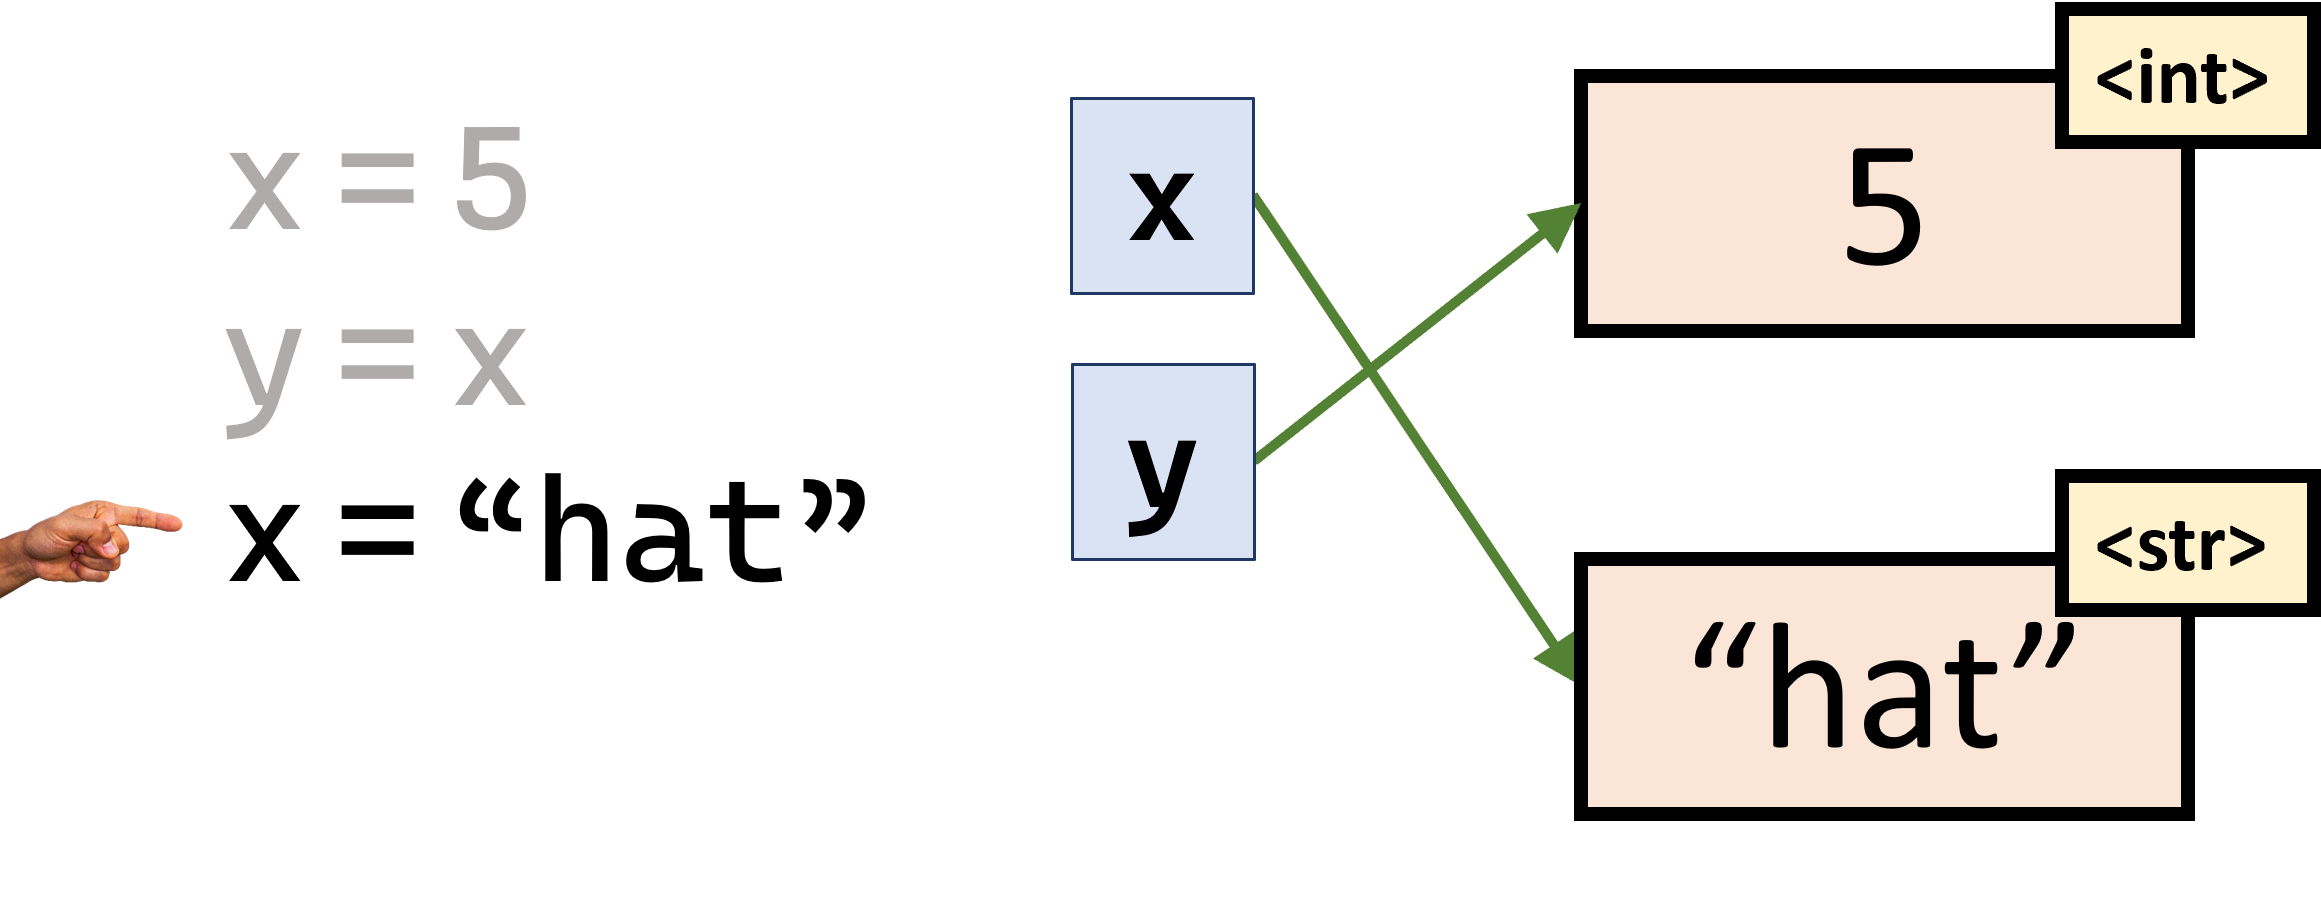
\includegraphics[width=0.8\textwidth]{pics/assignment2.png}
            \caption{Variable Assignment}
        \end{figure}
    \end{columns}
    
\end{frame}

\begin{frame}[fragile]{Variable Assignment}
    \begin{lstlisting}[style=colorful, language=Python]
>>> x = 20
>>> y = x
>>> x = "hello"
>>> print(y)
20
>>> print(x)
hello
    \end{lstlisting}
\end{frame}


\begin{frame}{Naming Variables}
    \begin{itemize}
        \item Variable names must start with a letter or an underscore
        \item The rest of the name can contain letters, numbers, and underscores
        \item Variable names are case-sensitive
        \item Variable names should be descriptive
    \end{itemize}
\end{frame}

\begin{frame}[fragile]{Reserved Keywords}
    \begin{lstlisting}[style=colorful, language=Python]
     >>> import keyword
     >>> keyword.kwlist      
    \end{lstlisting}
\end{frame} 

\begin{frame}
    \frametitle{Comparison Operators}
    \begin{itemize}
        \item Comparison operators are used to compare two values
        \item They return a boolean value (True or False)
        \item Common comparison operators include:
        \begin{itemize}
            \item \texttt{==} (equal to)
            \item \texttt{!=} (not equal to)
            \item \texttt{>} (greater than)
            \item \texttt{<} (less than)
            \item \texttt{>=} (greater than or equal to)
            \item \texttt{<=} (less than or equal to)
        \end{itemize}
    \end{itemize}
\end{frame}


\begin{frame}[fragile]{Python Quiz-1}
\begin{lstlisting}[style=colorful, language=Python]
>>> 5 == 5.0000
>>> 1+2 == 3 
>>> 9 > 8.999999999999999
>>> 6 // 3 == 6.0 / 3.0
\end{lstlisting}
\end{frame}

\begin{frame}[fragile]{Floating-Point Comparisons}
    \begin{itemize}
        \item Floating-point numbers can have precision issues due to their representation in memory.
        \item Comparisons involving equality can be affected by these precision issues.
        \item Example: \texttt{1.1 + 2.2 == 3.3} evaluates to \texttt{False} due to tiny inaccuracies.
        \item However, comparisons involving inequality are less likely to be affected.
        \item Example: \texttt{9 > 8.999999999999999} evaluates to \texttt{True}.
    \end{itemize}
    \begin{lstlisting}[style=colorful, language=Python]
>>> 1.1 + 2.2 == 3.3
False
>>> 9 > 8.999999999999999
True
    \end{lstlisting}
\end{frame}

\begin{frame}[fragile]
    \frametitle{Python Quiz-2}
    \begin{lstlisting}[style=colorful, language=Python]
>>> 5 != 5.0000
>>> True != False
>>> False < True
>>> "10" > "2"
    \end{lstlisting}
\end{frame}
\begin{frame}{What are Chained Comparisons?}
    \begin{itemize}
      \item Python allows multiple comparison operators to be chained together in a single expression.
      \item This creates a more readable and concise way to express complex comparisons.
      \item The comparisons are evaluated from left to right, and they are implicitly combined using the logical \texttt{and} operator.
    \end{itemize}
  \end{frame}
  
  \begin{frame}[fragile]{Example 1: Simple Range Check}
    \begin{itemize}
      \item Consider checking if a variable \texttt{x} is within a specific range.
      \item Without chained comparisons:
        \begin{lstlisting}[style=colorful, language=Python]
  if 10 < x and x < 20:
      # ...
        \end{lstlisting}
      \item With chained comparisons:
        \begin{lstlisting}[style=colorful, language=Python]
  if 10 < x < 20:
      # ...
        \end{lstlisting}
      \item Both are equivalent, but the chained version is more readable.
    \end{itemize}
  \end{frame}
  
  \begin{frame}[fragile]{Example 2: Multiple Comparisons}
    \begin{lstlisting}[style=colorful, language=Python]
  x = 5
  y = 10
  z = 15
  if x < y < z:
      print("x < y < z is True")
    \end{lstlisting}
    \begin{itemize}
      \item This checks if \texttt{x} is less than \texttt{y} AND \texttt{y} is less than \texttt{z}.
    \end{itemize}
  \end{frame}
  
  \begin{frame}[fragile]{Example 3: Equality and Inequality}
      \begin{lstlisting}[style=colorful, language=Python]
  a = 10
  b = 10
  c = 15
  if a == b < c:
      print("a==b<c is True")
      \end{lstlisting}
      \begin{itemize}
          \item This checks if \texttt{a} is equal to \texttt{b} AND \texttt{b} is less than \texttt{c}.
      \end{itemize}
  \end{frame}

